%%%
% Plantilla de Memoria
% Modificación de una plantilla de Latex de Nicolas Diaz para adaptarla 
% al castellano y a las necesidades de escribir informática y matemáticas.
%
% Editada por: Mario Román
%
% License:
% CC BY-NC-SA 3.0 (http://creativecommons.org/licenses/by-nc-sa/3.0/)
%%%

%%%%%%%%%%%%%%%%%%%%%%%%%%%%%%%%%%%%%%%%%
% Thin Sectioned Essay
% LaTeX Template
% Version 1.0 (3/8/13)
%
% This template has been downloaded from:
% http://www.LaTeXTemplates.com
%
% Original Author:
% Nicolas Diaz (nsdiaz@uc.cl) with extensive modifications by:
% Vel (vel@latextemplates.com)
%
% License:
% CC BY-NC-SA 3.0 (http://creativecommons.org/licenses/by-nc-sa/3.0/)
%
%%%%%%%%%%%%%%%%%%%%%%%%%%%%%%%%%%%%%%%%%

%----------------------------------------------------------------------------------------
%   PAQUETES Y CONFIGURACIÓN DEL DOCUMENTO
%----------------------------------------------------------------------------------------

%%% Configuración del papel.
% microtype: Tipografía.
% mathpazo: Usa la fuente Palatino.
\documentclass[a4paper, 11pt]{article}
\usepackage[protrusion=true,expansion=true]{microtype}
\usepackage{mathpazo}
\usepackage{amsthm}
\usepackage{graphicx}




% Indentación de párrafos para Palatino
\setlength{\parindent}{0pt}
  \parskip=8pt
\linespread{1.05} % Change line spacing here, Palatino benefits from a slight increase by default


%%% Castellano.
% noquoting: Permite uso de comillas no españolas.
% lcroman: Permite la enumeración con numerales romanos en minúscula.
% fontenc: Usa la fuente completa para que pueda copiarse correctamente del pdf.
\usepackage[spanish,es-noquoting,es-lcroman]{babel}
\usepackage[utf8]{inputenc}
\usepackage[T1]{fontenc}
\selectlanguage{spanish}


%%% Gráficos
\usepackage{graphicx} % Required for including pictures
\usepackage{wrapfig} % Allows in-line images
\usepackage[usenames,dvipsnames]{color} % Coloring code


%%% Matemáticas
\usepackage{amsmath}


%%% Bibliografía
\makeatletter
\renewcommand\@biblabel[1]{\textbf{#1.}} % Change the square brackets for each bibliography item from '[1]' to '1.'
\renewcommand{\@listI}{\itemsep=0pt} % Reduce the space between items in the itemize and enumerate environments and the bibliography



%----------------------------------------------------------------------------------------
%   TÍTULO
%----------------------------------------------------------------------------------------
% Configuraciones para el título.
% El título no debe editarse aquí.
\renewcommand{\maketitle}{
  \begin{flushright} % Right align
  
  {\LARGE\@title} % Increase the font size of the title
  
  \vspace{50pt} % Some vertical space between the title and author name
  
  {\large\@author} % Author name
  \\\@date % Date
  \vspace{40pt} % Some vertical space between the author block and abstract
  \end{flushright}
}

%% Título
\title{\textbf{Algoritmos voraces (greedy) II}\\ % Title
Travelling salesman problem} % Subtitle

\author{\textsc{Ignacio Mas Mesa,\\Braulio Valdivielso Martínez} % Author
\\{\textit{Universidad de Granada}}} % Institution

\date{\today} % Date



%----------------------------------------------------------------------------------------
%   DOCUMENTO
%----------------------------------------------------------------------------------------

\begin{document}

\maketitle % Print the title section

%% Resumen (Descomentar para usarlo)
\renewcommand{\abstractname}{Abstract} % Uncomment to change the name of the abstract to something else
\begin{abstract}
En esta ocasión vamos a continuar nuestro estudio de los algoritmos voraces (greedy), ahora aplicados a uno de los problemas más famosos de las ciencias de la computación: el problema del viajante de comercio (TSP, por sus siglas en inglés). El problema consiste en, dada una lista de ciudades (en nuestro caso puntos en un plano) y una métrica (asumimos la euclídea, pero pueden ser pesos de las aristas de un grafo) encontrar la ruta más corta que pasa exactamente una vez por cada ciudad (volviendo a la de partida).

Este problema ha sido estudiado durante casi cien años desde su planteamiento en 1930, pero sigue siendo interesante en tanto que es un problema NP-hard, i.e., cualquier problema en NP puede ser reducido a él en tiempo polinómico.
\end{abstract}

\vspace{30pt} % Some vertical space between the abstract and first section


%% Índice
  \tableofcontents

\pagebreak

%%% Inicio del documento

\section{Problema}
Nuestro problema es el siguiente:
\begin{quote}
Dada una lista de ciudades (puntos del plano ${\mathbb Q}^2$) encontrar la ruta más corta que pasa exactamente una vez por cada ciudad volviendo a la de partida usando como distancia la euclídea.
\end{quote}

\section{Soluciones}
\subsection{Solución greedy: vecino más cercano}
\makebox[\textwidth]{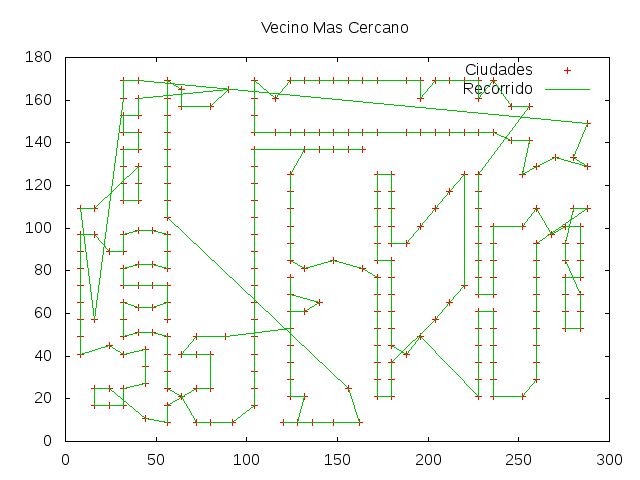
\includegraphics{./results/Vecino Mas Cercano.png}}
El primer algoritmo es trivial: empezamos en una ciudad cualquiera y, en cada paso, visitamos la ciudad más cercana.

Pese a lo simple de esta solución, en el caso medio puede encontrar rutas sólo un 25\% más largas que la óptima. Sin embargo, es cierto también que se pueden encontrar ejemplos de disposiciones en las que este algoritmo encuentra la peor ruta posible.

\subsection{Solución con inserción}
\makebox[\textwidth]{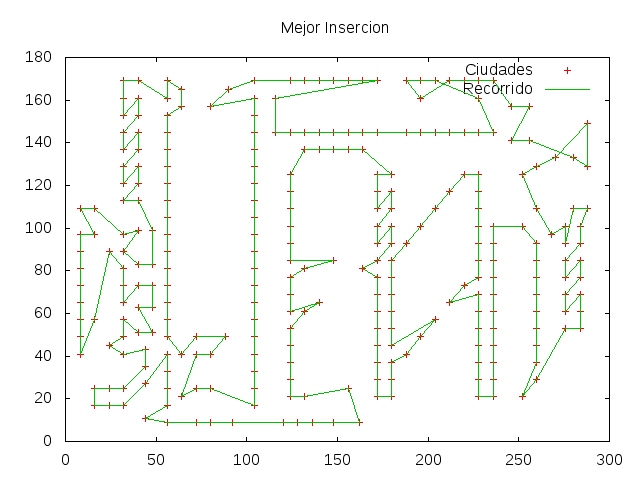
\includegraphics{./results/Mejor Insercion.png}}
El segundo algoritmo también es, sensu lato, greedy, aunque más sofisticado que el anterior. Tomamos un par de ciudades cualesquiera y, en cada paso, comprobamos cuánto costaría insertar cada ciudad no visitada en cada posición posible de la ruta, y tomamos el mínimo. 

Para calcular cuánto nos \"cuesta\" insertar una ciudad en un cierto punto simplemente sumamos la distancia de la nueva ciudad a la que va antes, la distancia a la que va después y restamos la distancia entre las ciudades anterior y posterior.

\subsection{Solución Lin-Kernighan (2-opt)}
\makebox[\textwidth]{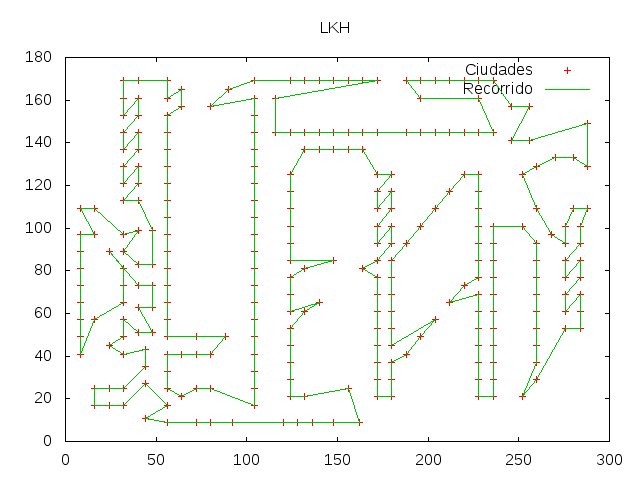
\includegraphics{./results/LKH.png}}
La tercera solución que proponemos es la de usar la heurística de Lin-Kernighan en su versión más simple. Esta heurística es un algoritmo genético que toma una permutación de las ciudades y, en cada paso, elimina $k$ aristas no contiguas, de forma que nos quedan $k$ \textit{clusters}. Ahora los pegamos entre sí (debe quedarnos de nuevo un ciclo conexo) en el orden que queramos, y, si el coste actual de la permutación es menor, nos la quedamos como solución actual.

Este proceso se puede repetir un número indefinido de veces, ya que a priori no sabemos cuál es la solución óptima como para marcar un límite de bondad de la solución en el que detenernos.

Para el caso que nos ocupa hemos tomado como permutación inicial la generada por la heurística anterior, de forma que mantenemos el orden de eficiencia polinómico obteniendo soluciones aún mejores; y $k=2$, que básicamente le da la vuelta a una porción de la permutación, e iteramos $N^2$ veces, donde $N$ es el número de ciudades. Así, es muy rápido calcular si una cierta mutación del recorrido es beneficiosa o no (dos sumas y dos restas), pero podemos conseguir muy buenos resultados.

Para el caso que nos ocupa hemos tomado $k=2$, que básicamente le da la vuelta a una porción de la permutación, e iteramos $N^2$ veces, donde $N$ es el número de ciudades. Así, es muy rápido calcular si una cierta mutación del recorrido es beneficiosa o no (dos sumas y dos restas). Para obtener mejores resultados, hemos hecho que nuestro algoritmo 2-opt parta de la solución encontrada por el algoritmo de mejor inserción.

\section{Comparación de los algoritmos}
Para poder comprobar la bondad de nuestros algoritmos, se nos suministraron múltples sets de datos (procedentes de TSPLib) con sus respectivas rutas óptimas. De aquellos mapas que se nos dieron, tuvimos que comprobar en la documentación de TSPLib cuáles de esos mapas estaban diseñados con la intención de usar la distancia euclídea, que es la que nos ocupa. Una vez conseguimos eliminar los mapas no preparados para nuestro trabajo, llegamos a un set de datos con 17 mapas, sobre el que podíamos ejecutar nuestros algoritmos y comparar los costes obtenidos con los de las soluciones óptimas.

Tras numerar los mapas por orden alfabético y ejecutar los algoritmos llegamos a los siguientes resultados.


\makebox[\textwidth]{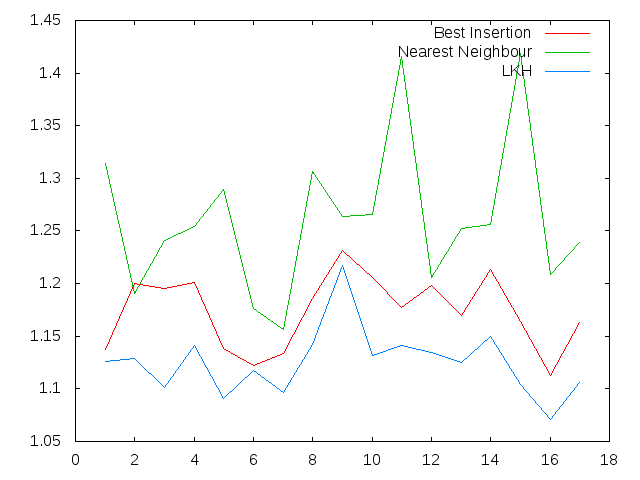
\includegraphics{./results/algorithm-comparison}}


Comprobando el comportamiento individual de los algoritmos llegamos a los siguientes datos:
\begin{itemize}
	\item Vecino más cercano: 26.204\% más costoso que el óptimo.
	\item Mejor inserción: 17.349\% más costoso que el óptimo
	\item LKH: 12.506\% más costoso que el óptimo.
\end{itemize}

\section{Conclusiones}
Tras realizar esta práctica, hemos llegado a los resultados esperados. La heurística más sencilla y más ingenua es la que peores resultados ha obtenido en esta ocasión. En segundo lugar encontramos la heurística de mejor inserción, y en primer lugar la LKH. Teniendo en cuenta la implementación que hicimos del último algoritmo, era obvio que esto sucedería de esta forma, ya que se partía de la solución de la mejor inserción, y de ahí solo podía mejorar.

\end{document}